\section{Results and Analysis}
\label{sec:results and analysis}

\subsection{Results}

The runs' performance are evaluated on this year's relevance qrels, provided by CLEF, built performing top-5 pooling on the runs delivered by all participants. \citep{bondarenko:2022e}

In table \ref{tab:compare-results} we show, for each run, the NDCG@5 score obtained during model selection and the respective NDCG@5 score obtained with CLEF's relevance qrels.

\begin{table}[t]
	\caption{Model and CLEF's qrels scores}
	\label{tab:compare-results}
	\centering
	\begin{tabular}{|c|c|c|}
	\toprule
	\# & selection NDCG@5 & Final NDCG@5 \\
	\midrule
	1 & 0.3830 & 0.3828 \\
	2 & 0.3756 & 0.3688 \\
	3 & 0.3313 & 0.2937 \\
	\hline
	4 & 0.4140 & 0.4497 \\
	5 & 0.4258 & 0.4461 \\
	6 & 0.4366 & 0.4746 \\
	7 & 0.4548 & 0.4896 \\
	\hline
	8 & 0.4015 & 0.4376 \\
	9 & 0.4759 & 0.5226 \\
	10 & 0.4823 & 0.5042 \\
	\hline
	11 & 0.2634 & 0.2289 \\
	12 & 0.3654 & 0.4088 \\
	13 & 0.4525 & 0.4535 \\
	14 & 0.4674 & 0.4939 \\
	\hline
	\textit{\textbf{15}} & 0.4873 & 0.5466 \\
	\hline
	16 & 0.8549 & 0.6098 \\
	17 & 0.8552 & 0.6036 \\
	\hline
	18 & 0.5867 & 0.5812 \\
	19 & 0.5392 & 0.5772 \\
	\textit{\textbf{20}} & 0.5714 & 0.6362 \\
	\textit{\textbf{21}} & 0.8606 & 0.6954 \\
	22 & 0.8323 & 0.6669 \\
	\hline
	\textit{\textbf{23}} & 0.7521 & 0.6681\\
	\textit{\textbf{24}} & 0.7450 & 0.7089\\
	\bottomrule
\end{tabular}
\end{table}

The scores are close to the ones obtained in model selection and all choices done are confirmed by the final results.

The only runs that differ much from the ones in the model selection are, as expected due to the mentioned overfitting, the ones that use Relevance Feedback.
These runs still have a better score than other run obtained before reranking, but they don't differ from them as much as they did earlier.

The runs obtained through RRF also suffer a decrease in score, also due to the previous partial overfitting deriving from RF runs.

As expected reranking improved the performance of all runs, included RF and RRF runs.

The only result hinted in the model selection that we didn't expect to turn out to be true was that Porter stemmer slightly worsened the score when applied to RF runs.

The best performing run is run 24, the reranked RRF run.

\subsection{Statistical Analysis}

All the following statistical analysis have been obtained using CLEF's relevance qrels.

In the analysis, to produce better results, when a run retrieves no documents for a topic the NDCG@5 score is set to 0, while earlier that topic was not considered in the average NDCG@5 in the run, therefore results are worse than to the ones observed earlier for those runs (8, 9, 10, 18).

First we wanted to check if the runs were significantly different between them, in order to do so we have used Tukey's HSD test \citep{Tukey}, with $\alpha=0.05$: Figure~\ref{fig:multcomp}

\begin{figure}[h]
	\centering
	\includegraphics[width=0.9\textwidth]{figure/Multcomp.pdf}
	\caption{Multiple comparison of Tukey's HSD test}
	\label{fig:multcomp}
\end{figure}

In particular run 24 is highlighted, to show how it significantly differs from all runs not using RF or reranking (runs 1 to 15)

Then we produced a boxplot graph showing, for each run, the NDCG@5 score of each topic on the Y axis, ordered by average NDCG@5: Figure~\ref{fig:runs-boxplot-ordered}

\begin{figure}[h]
	\centering
	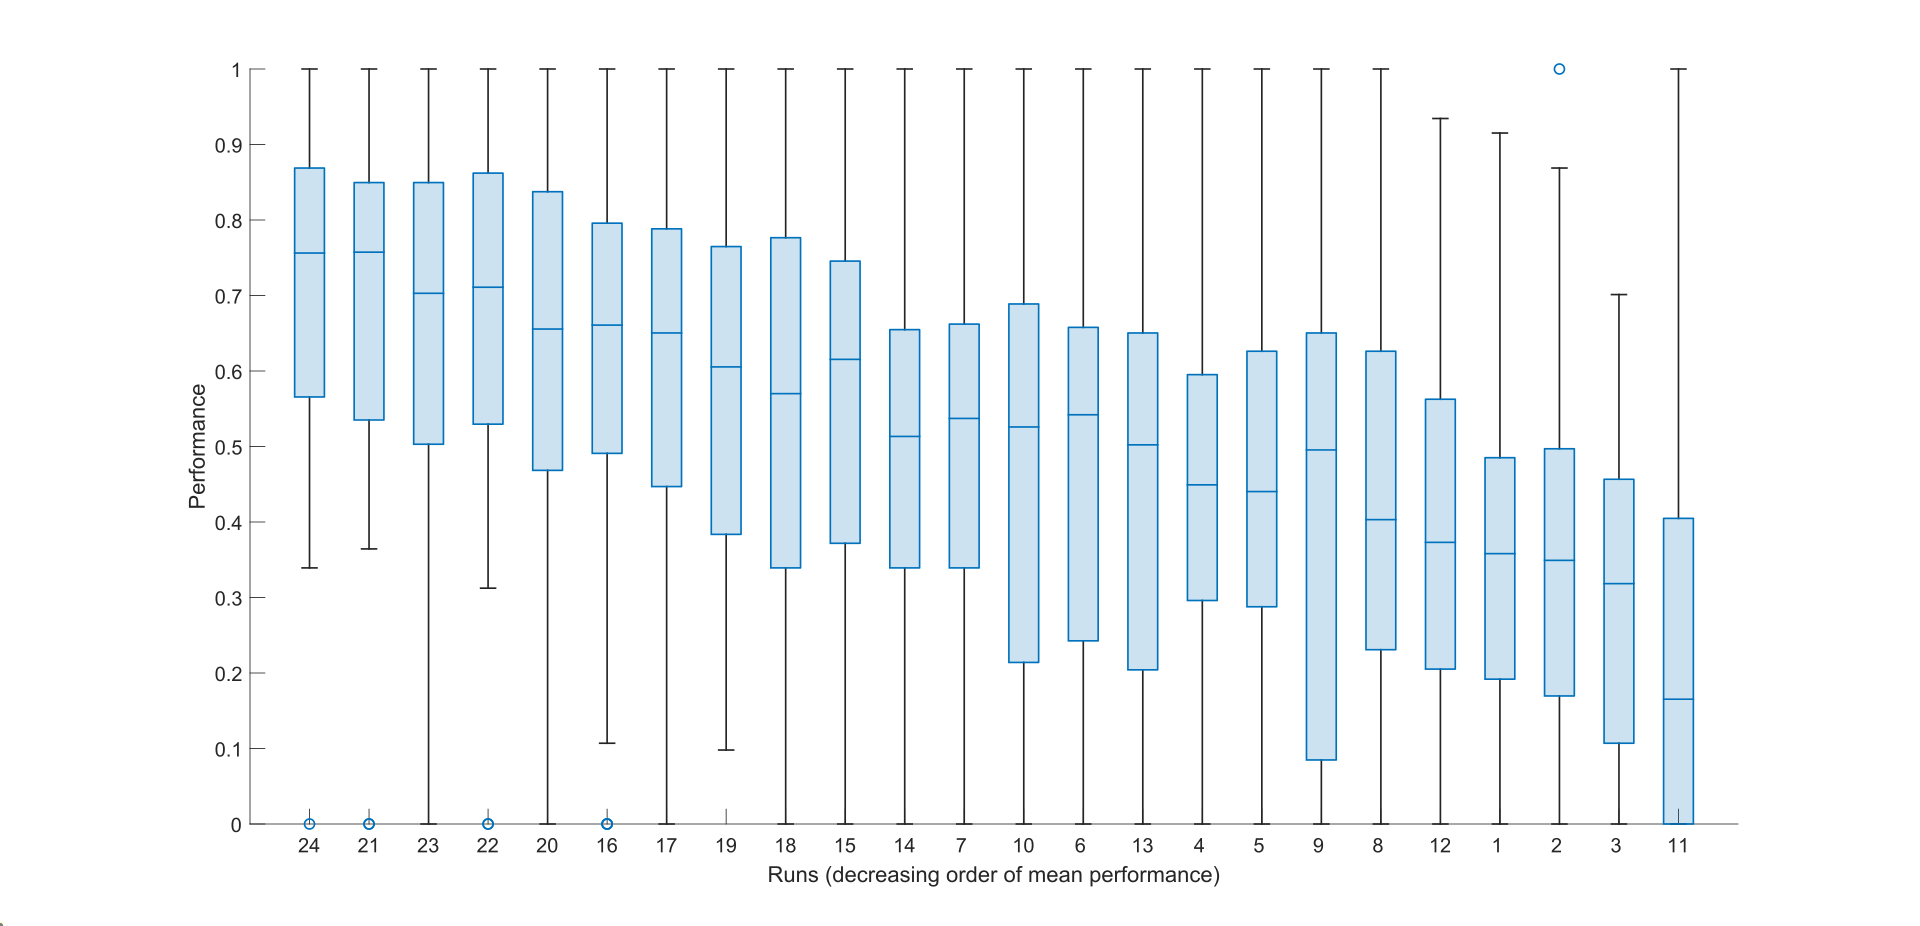
\includegraphics[width=0.9\textwidth]{figure/RunsBoxPlotOrdered.pdf}
	\caption{Run's Boxplot ordered by NDCG@5}
	\label{fig:runs-boxplot-ordered}
\end{figure}

All runs have a very similar interquartile range and all runs, except run 19, have a score equal to 0 for at least one topic.

Following these results we also got interested in finding out the difference by topics, to see what type of topic we had a poor performance on: Figure~\ref{fig:topics-boxplot-ordered}

\begin{figure}[h]
	\centering
	\includegraphics[width=0.9\textwidth]{figure/TopicsBoxPlotOrdered.pdf}
	\caption{Topics's Boxplot ordered by NDCG@5}
	\label{fig:topics-boxplot-ordered}
\end{figure}

The run got their worse results on topics 43, 86 and 77, which are respectively:
\begin{itemize}
	\item Should I prefer a Leica camera over Nikon for portrait photographs?
	\item I am planning to buy sneakers: Which are better, Adidas or Nike?
	\item Is it healthier to bake than to fry food?
\end{itemize}
The problem we found in particular with these topics is, for the first two, that a lot of documents retrieved were ads, and for the last one that a lot of documents retrieved were just recipes that bake or fry food.

Due to these results we believe in future work it might be useful to add  to the search keywords or shingles offering comparison (e.g. "versus", "compared to", "against"), since comparison between two items is intrinsic to the task.

We also decided to check the difference in performance in different topics between our best run and the third and second best, again to check the reason for the dip in performance in specific topics: Figure~\ref{fig:diff24-21} Figure~\ref{fig:diff24-23}

\begin{figure}[h]
\centering
\includegraphics[width=0.9\textwidth]{figure/rundiff24-21.pdf}
\caption{Difference in performance by topic in runs 24 and 21}
\label{fig:diff24-21}
\end{figure}

When comparing run 24 to run 21 the performance is noticeably worse, with a difference of 0.5, for topic 9:  "Why is Linux better than Windows?"

This top is however is one of the worse performing topic among all runs and at the same time has the largest interquartile range.

Going more in depth we find, rather than the weaknesses of run 24, a proof to the strength of Relevance Feedback: in fact, in this specific topic in general the documents retrieved often display people talking about one of the two objects, Relevance Feedback runs instead excel because they look for keywords, that are very often used when comparing the two objects, like for example "price", "safety", "open" and "source".\newline

\begin{figure}[h]
	\centering
	\includegraphics[width=0.9\textwidth]{figure/rundiff24-23.pdf}
	\caption{Difference in performance by topic in runs 24 and 23}
	\label{fig:diff24-23}
\end{figure}

The comparison between run 24 and 23 is particularly interesting, since the first is the reranked version of the second. A noticeable dip in performance from run 23 to run 24 can be seen in topics 30 and 26:
\begin{itemize}
	\item Should I buy an Xbox or a PlayStation?
	\item Which is a better vehicle: BMW or Audi?
\end{itemize}
We decided to go in depth to find out the reason of the worse performance in topic 30 (Xbox vs. Playstation) by manually checking the top-5 document retrieved for each and their relevance score in qrels.

The main reason for the difference is that most of the relevant document for run 23 are formed mainly by short ads (in the format "item on sale - price"), but also contained a very short phrase that was relevant to the topic. These document when reranking suffer a big penalty due to their low sentence quality.

Instead, in run 24 we found a document that is uniquely an ad (which was unexpected as we thought that reranking with sentence quality was a very good way to push ads down in the ranking), however this document was a well written ad, consisting of a company advertising their business that sold consoles, therefore it's sentence quality score is high.

A problem we found in this in depth analysis is that some documents (e.g. clueweb12-1810wb-39-31830\_\_\_3, clueweb12-1808wb-28-21892\_\_\_11) were poorly scored, since these documents were comprised of only ads, containing no relevant information at all to the topic, but still were scored as partially relevant.
Finding these two blatant mistakes in only 8 documents manually checked (two document are present in both runs) raises concerns on the reliability of the relevance scores delivered by CLEF.